\chapter{Application: font glyph generation}\label{chap:training}
To demonstrate our end-to-end SVG generation method, we train the model architecture described in Chapter~\ref{chap:architecture} on a dataset of font glyphs.

\section{Dataset}\label{sec:font-data}
Our dataset of font faces is downloaded from a GitHub repository containing all fonts available on Google Fonts (\url{https://github.com/google/fonts}).
The dataset contains 2552 font faces total from 877 font families.
A breakdown of font types for the 877 font families can be found in Table~\ref{tbl:fonttypes}.

\begin{table}[h]
\centering
\caption[A breakdown of font types in the Google Fonts dataset]
    {The 2552 font faces in the Google Fonts dataset are from 877 total font families.
    Each font family can be classified as one of the following categories, with the ``display'' category encompassing bold fonts of a wide variety of styles that can be used as title text.
    Here, we report the counts of font families in the dataset belonging to each type.\label{tbl:fonttypes}}
\begin{tabular}{c c c c c}
\toprule
    Serif & Sans serif & Display & Handwriting & Monospace \\ \midrule
    180 & 249 & 296 & 135 & 17
\end{tabular}
\end{table}

All font faces are downloaded as TTF files then converted to SVG format using the FontForge command-line tool\footnote{\url{https://fontforge.github.io}}.

\section{Training}
\section{Results}
\subsection{Quantitative results}
\begin{figure}[t]
	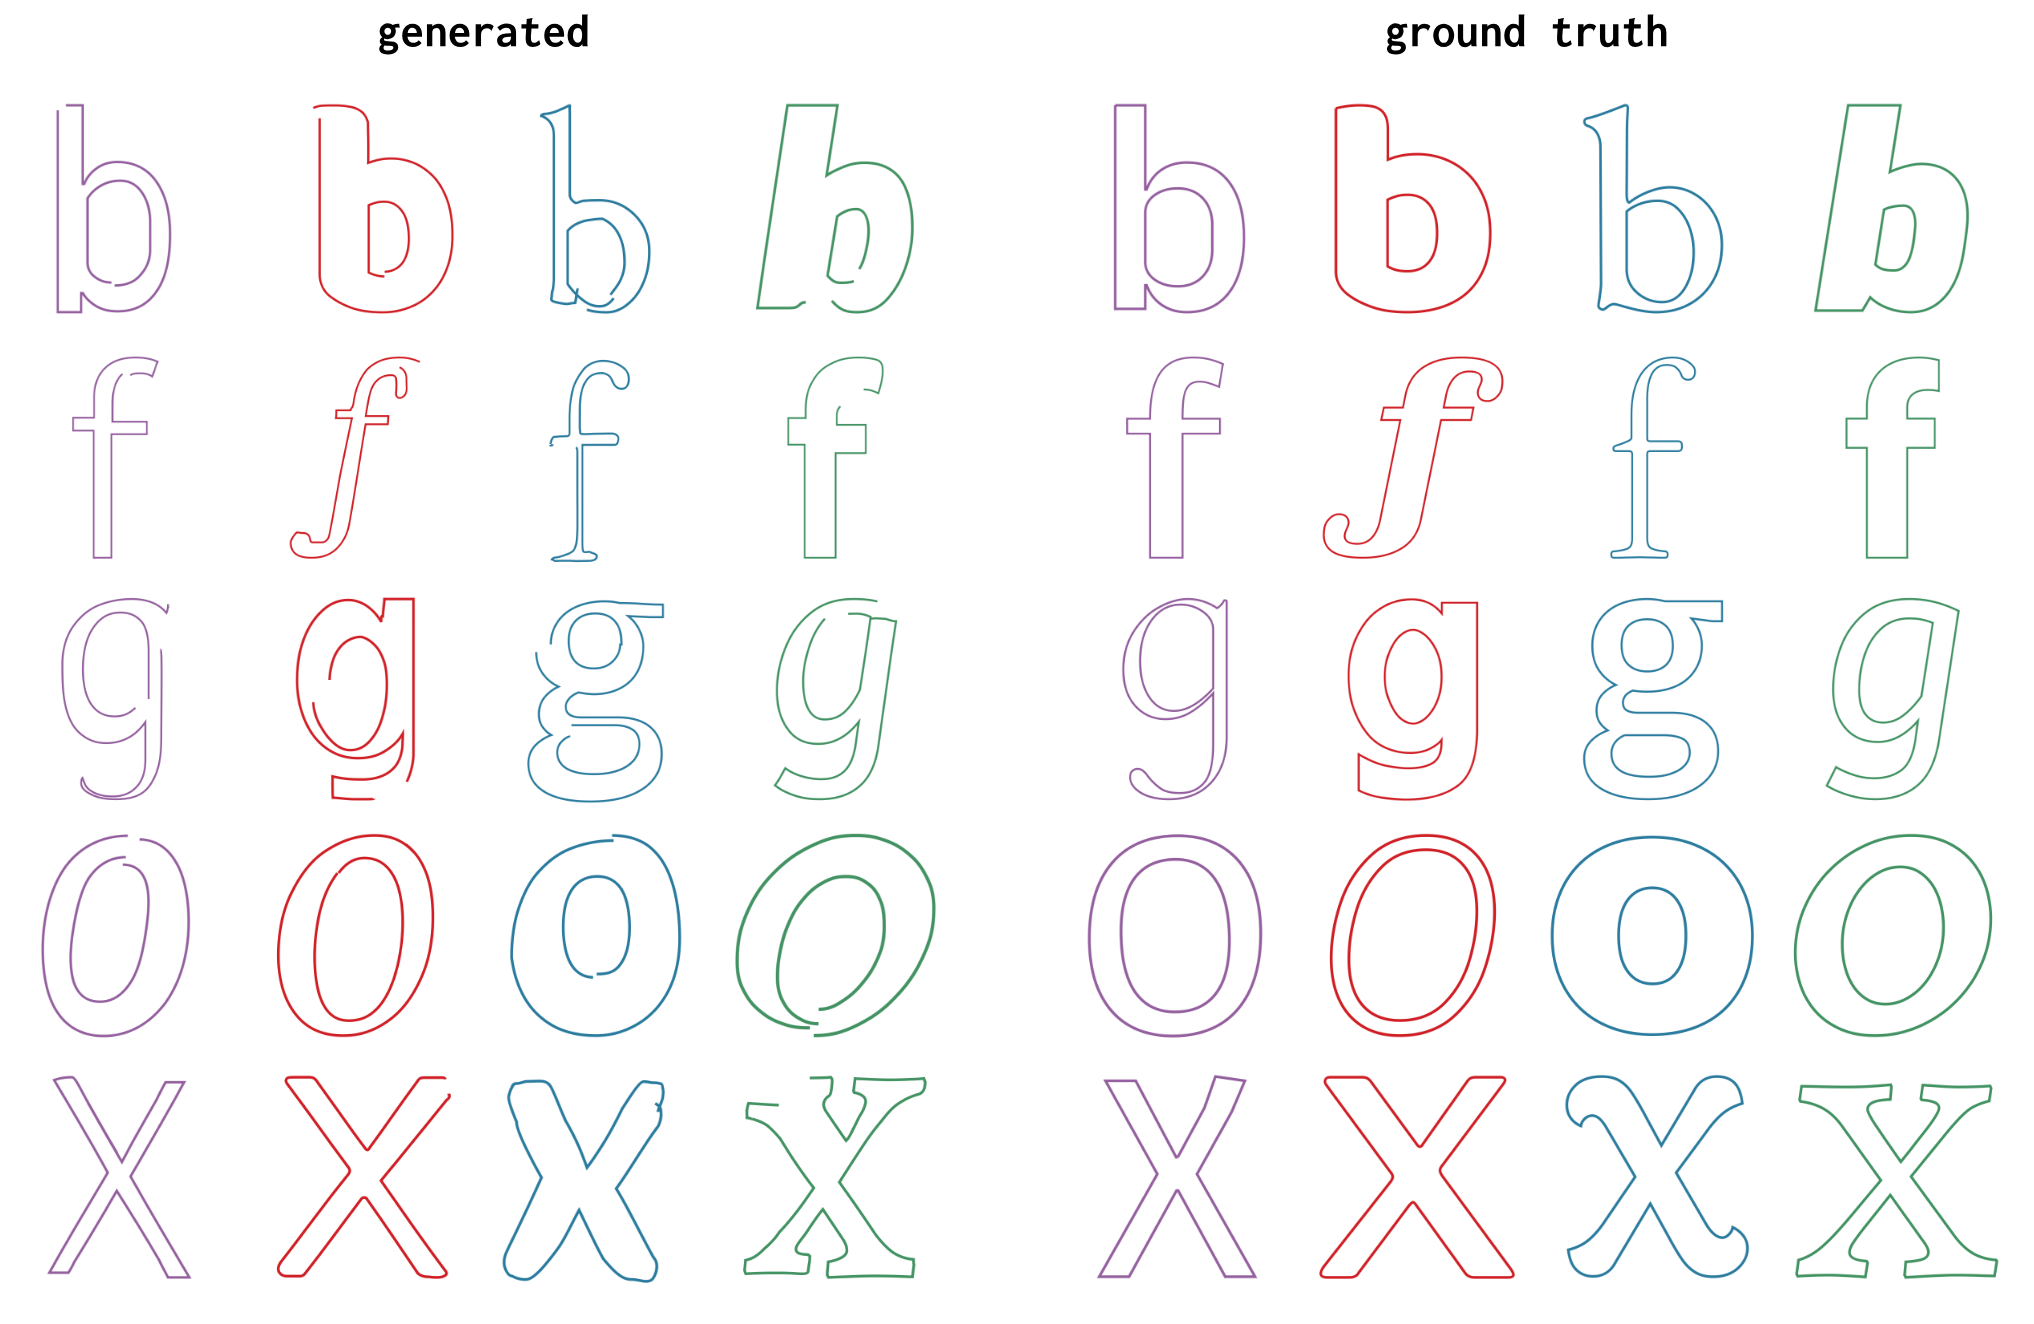
\includegraphics[width=\textwidth]{figures/font_gen}
    \caption[Visual results of training \TODO{blah}]
    {\TODO{replace}\label{fig:font_gen}}
\end{figure}

\subsection{Qualitative results}
\TODO{common failures}
\TODO{vector interpolation}

